\chapter{関連研究}
%20191222 推敲1回目済み
\label{chap:smile}

本章では, はじめに人の表情についての関連研究ついてまとめる.
ついで, 情報学の分野における表情, 特に笑顔に関する先行研究の例を取り上げる.
最後に, 本研究において取り扱う笑顔について定義する.

\section{人と表情に関する研究}
本節では, 人の表情についての関連研究および表情と人間関係の関連性の2つについてまとめる.
\subsection{人の表情について}
Ekmanは感情を表す普遍的な基本表情があるという理論を提唱した.
その表情は7つに分類され, 怒り,嫌悪,恐怖,驚き,悲しみ,幸福に中立な表情を加えたものである\cite{ekman}.
\begin{figure}[htbp]
    \begin{center}
       \fbox{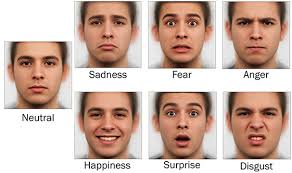
\includegraphics[width=150mm,bb=0 0 292 173]{universal_facial_expressipn.jpeg}}
    \end{center}
    \caption{人間の普遍7表情}
    \label{fig:universal_facial_expression}
\end{figure}
佐藤らが日本人に対して, Ekmanの基本表情が適用されるのかを実験した際には,
部分的にしか日本人には適応されないことがわかったが, 驚きと幸福に関する基本表情は日本人にも
適合することが証明されている.\cite{JapaneseFacialExpression}
\begin{figure}[htbp]
    \begin{center}
       \fbox{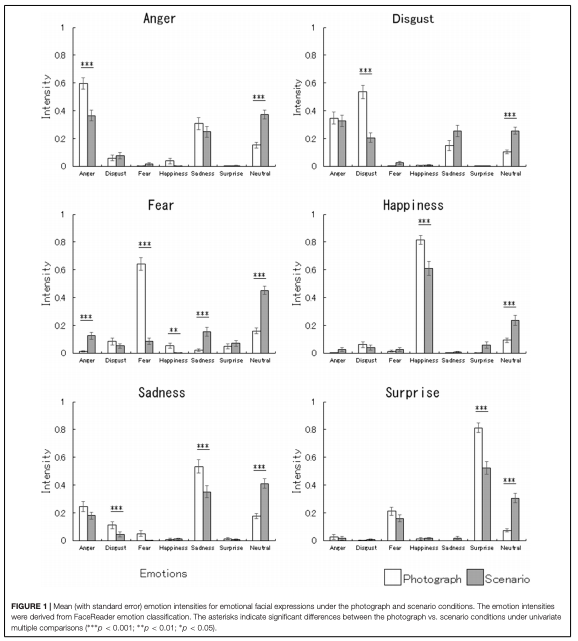
\includegraphics[width=100mm,bb=0 0 578 641]{emotion_graph.jpg}}
    \end{center}
    \caption{日本人の表情判断グラフ}
    \label{fig:JapaneseFacialExpression}
\end{figure}

\subsection{人間関係と表情について}
顔には年齢, 性別, 人種などの生物学的属性に加え, 口の動きからの発話情報, その人物の人となり,
感情, 意図, 関心などを読み取ることが可能である\cite{role_facialexpression_in_communication}.
人はコミュニケーションをとる際に, 会話の内容などの言語コミュニケーションに加え,
表情などの非言語コミュニケーションが行われる.
非言語コミュニケーションとは, 言葉を使わないコミュニケーションのことを指し,
Mehrabianによればコミュニケーションにおいて,非言語コミュニケーションは印象情報の93\% を占める\cite{rule_of_Mehrabian}.
ゆえに, コミュニケーションにおいて会話内容よりも, 人の見た目や表情に意識が向く.
表情, 特に笑顔はコミュニケーションをとる際に重要な役割を担っている.


\section{情報技術と笑顔に関する研究}
近年, 情報処理技術を用いて人の表情分析の研究が進められている.
SONYが開発し, デジタルカメラ Cyber shotに組み込まれているスマイルシャッターは笑顔検出技術が,
システム搭載されている例である.
現在, 実用化が進んでいるが, より笑顔を検出する精度や速さが求められている.

\begin{figure}[htbp]
    \begin{center}
       \fbox{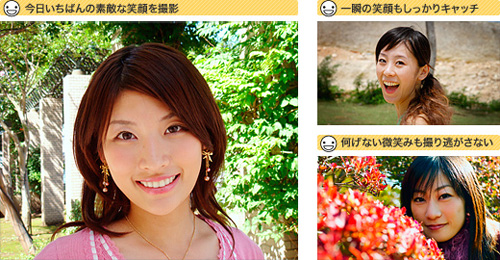
\includegraphics[width=150mm,bb=0 0 500 260]{sony_smile_shutter.jpg}}
    \end{center}
    \caption{SONYスマイルシャッター}
    \label{fig:sony_smile_shutter}
\end{figure}

Eduardらは口角をベースとした笑顔検出器を作成し,
既存の検知方法よりも速く笑顔の検出を可能にする手法の提案をしている\cite{EduardRoyce}.
人の笑顔を顔のパーツ, 特に目や口元, 頬の動きを判断材料として, 画像処理技術および機械学習を用いて自動的に笑顔を検出するような研究が数多く行われている.
他にも表情に現れる感情と, 実際に抱いている感情との違いを検出するような研究も行われている.
実際に人同士でも相手の内面状態を知ることは非常に難しい. 不快感を抱いていたとしても 相手に悟られないように笑顔を作るなど表情と感情が一致しないケースも数多くある.
I Gede Aris Gunadiらは,画像から機械学習を用いた作り笑顔を検出する研究\cite{IGedeArisGunadi}, Neeleshらは動画を用いて作り笑顔の検出\cite{NeeleshBhakt}を行うなど人の表情と内面状態との乖離を解消するような研究も進んでいる.
上記のように,先行研究においては笑顔のシーン単体に対して,処理を行い表情分析を行うものが多い.
人の表情は断片的なものではなく連続的なものである.
動画の分析を行う先行研究は映像から内面を推定する研究が主流であり,
中立の表情から笑顔になる過程について分析する研究はほとんど行われていない.
より人間の表出表現を正確に, 繊細に分析する際には連続的に表情の流れの中で分析する必要がある.


\section{本研究において取り扱う笑顔}
本研究では, 笑顔を内面の感情ではなく表情のみを取り扱う. %この理由を述べる(修正)
%心理学の分野においてWilliam Jamesは, 幸せだから笑うのではない笑うから幸せなのだ \cite{geary2006world} と述べている.
Niedenthalは初対面において本当の笑顔と作り笑顔の違いを見分けることは難しいことを述べることに加え,
人間は比較によって本当の笑顔か作り笑顔か判断をする. もし自分が相手が笑っていると判断した場合には
作り笑顔でも本当に笑顔か関係なく笑顔に対する印象の効力が発揮されると述べている\cite{niedenthal2010simulation}.
さらに表情の筋肉は無意識のうちに動きの癖が反映されており, 笑顔を自分の意思で作ろうとした時も普段の笑い方と
同じような筋肉が動くため,全ての表情には自分の内面属性・性格は反映されていると考えためである.

% https://www.huffingtonpost.co.uk/2013/10/07/fake-smile-real-smile-the-difference_n_4056325.html?guccounter=1&guce_referrer=aHR0cHM6Ly93d3cuZ29vZ2xlLmNvbS8&guce_referrer_sig=AQAAAHRxMuHbc9JLsBpPaSLGACzwJyP5Okg7CSdEx3S-Q54pkKwm1WJcHMwiSAcvPt8Ehc0P9aD_x_XP3MAomejqxmb6_C7xJr_ymaRInBPD2otliZTNsnNAVgO2WYW_LMw8kJ-YPwac-dmnET60IoHmkkox_dPt3c7mxeZguZYCe_Bk
%メモ
% https://visionary-mind.com/smile/


笑顔の作り方を分析し, 表出表現による自分の表情と相手の表情への嗜好判断を行う.
笑顔の分析オープンソースであるOpenFaceの中に含まれる, Facial Action Unitを用いて行う.
OpenFaceとはTadasらCambridge University, MultiCamp Labが作成した表情分析を行うためのツールである.
Facial Action Unit(以下FAUとする)は,Paul Ekman,Wallace Friesenらによって1978年に開発された分析ツールかつ表情理論に基づいたFacial Action Coding System
を使って,客観的に顔の動きをデータとして取得することのできる基本動作を定義したものである.
FAUにおいて,笑顔のunit番号は6(眼窩部眼輪筋),7(眼瞼部眼輪筋),12(大頬骨筋),25(翼突筋+顎二腹筋)である.
この4つのUnitを使用して笑顔の分析を本研究では行う.

\begin{figure}[htbp]
    \begin{center}
       \fbox{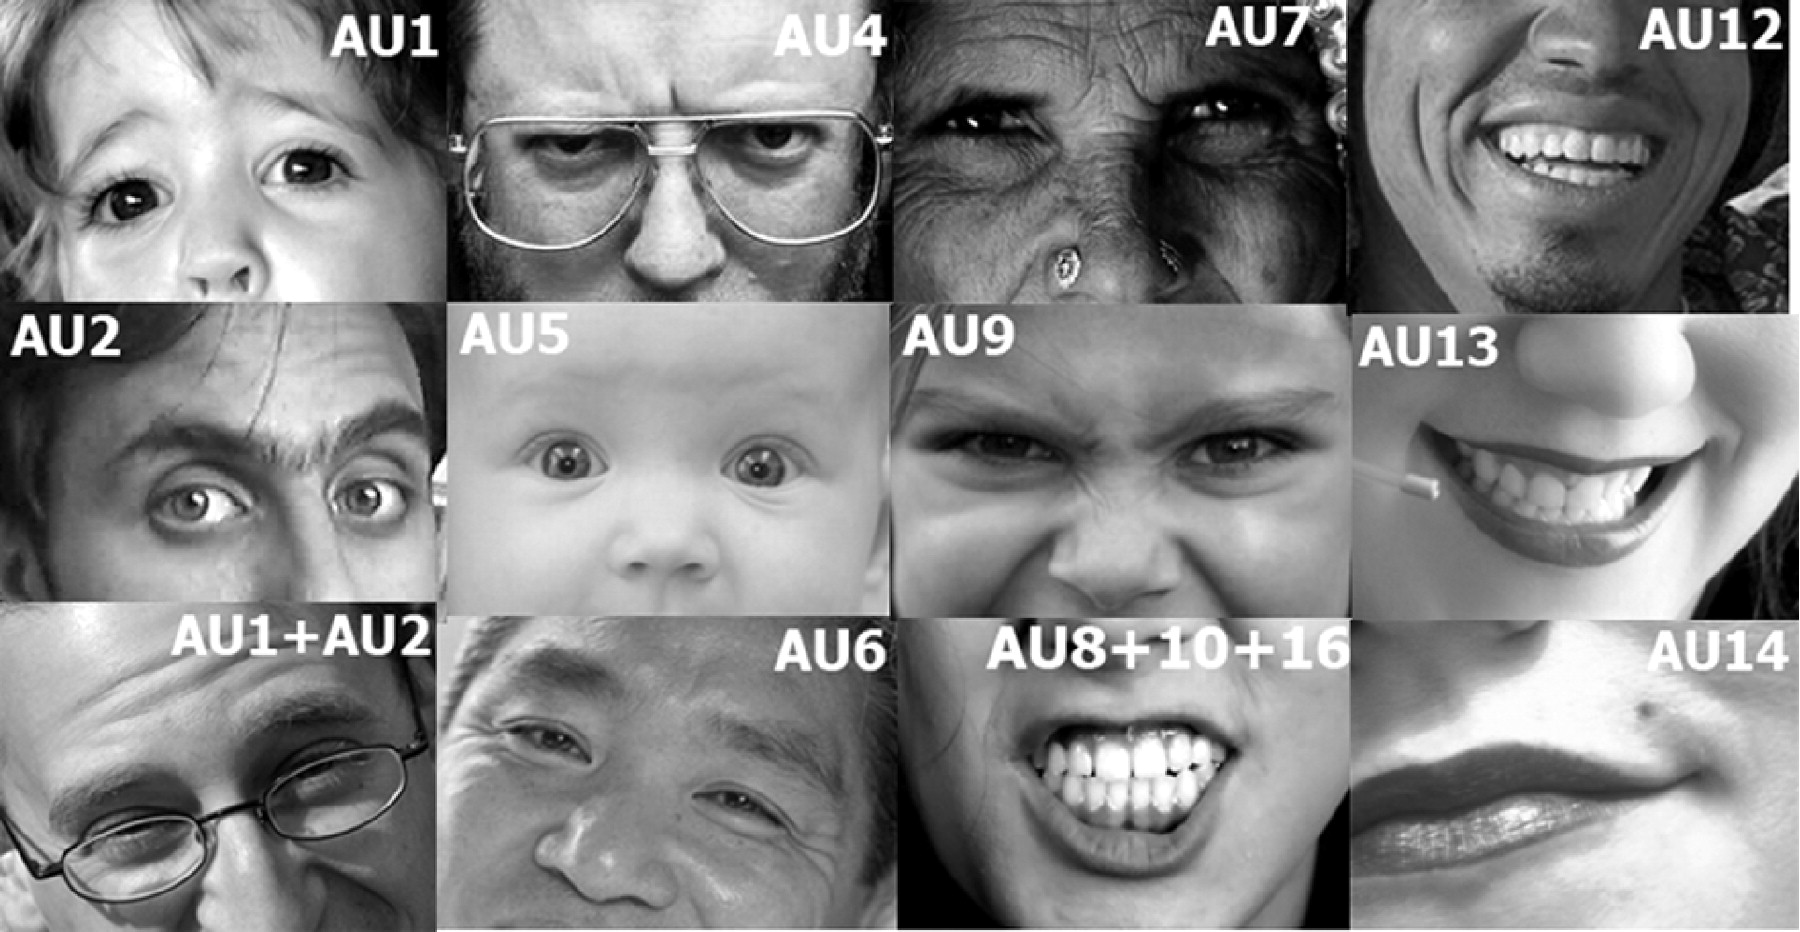
\includegraphics[width=150mm,bb=0 0 1800 932]{faus.jpg}}
    \end{center}
    \caption{Facial Action Unit例}
    \label{fig:faus}
\end{figure}

\begin{figure}[htbp]
    \begin{center}
      \fbox{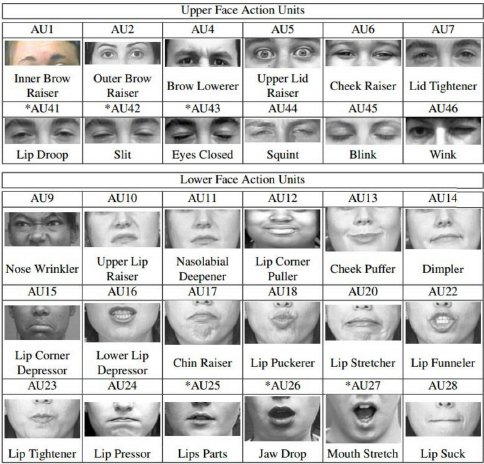
\includegraphics[width=150mm,bb=0 0 484 464]{faus2.jpg}}
    \end{center}
    \caption{Facial Action Unitの種類}
    \label{fig:faus2}
\end{figure}


\section{まとめ}
本章では, 現在行われている人の表情, 特に笑顔についての先行研究について整理した.
ついで, 本研究で扱うFacial Action Unit を用いて判断する笑顔について定義した.
次章では本研究において使用する, Delta Smile Facial Survey Analyzer のシステムの概要および特徴について述べる.
